\chapter{Optimisation of GEOS-Chem Predictions of Mercury Concentrations in the Atmosphere}
\section{Background}

high Hg emission ASGM Hg emissions can be estimated by leveraging simulations of Hg in the atmosphere generated by the GEOS-Chem model and observation data from long range Hg monitoring stations. By combining our top-down method with existing bottom-up data, we improve estimates of Hg emissions from ASGM activities, using Peru and the Madre de Dios region of South America as case studies.

\section{Methods}

\subsection{Modification of Mercury Inventories}
\begin{flushleft}
The GEOS-Chem Hg model takes the emissions inventory such as those shown on Figure \ref{fig:Hg_inventories} as an input and output the Hg concentration in the atmosphere that results from the input emissions. Moreover, the Hg concentration output is directly proportional to the amount of input emissions. 
\end{flushleft}
\begin{figure}[H]
  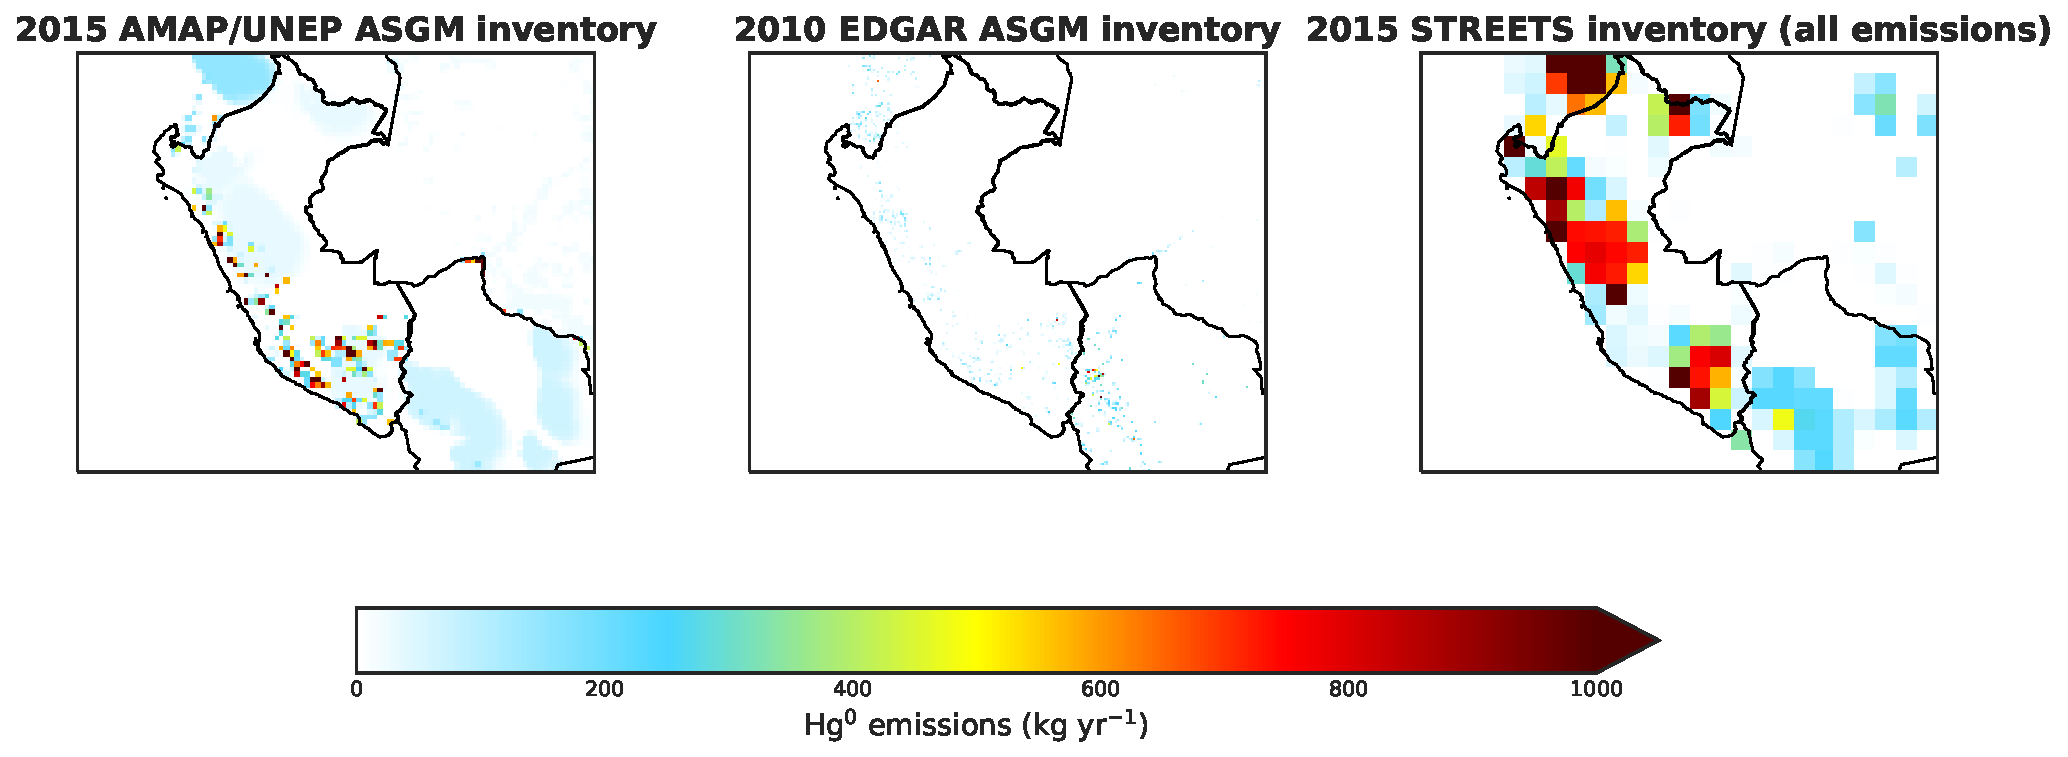
\includegraphics[width=\textwidth]{templates/figures/Peru_Maps/Hg_inventories.pdf}
  \centering
  \caption{Comparison of different Hg emission estimates by different global inventories}
  \label{fig:Hg_inventories}
  
\end{figure}
\FloatBarrier
\begin{flushleft}
The GMA 2018 ASGM emissions estimates for the year 2015 were used in the all the GEOS-Chem simulations we carried out. The  from individual grid boxes in the case study region as seen in Figure \ref{fig:GMA2018} were scaled and then used as input to the GEOS-Chem model. The emissions were scaled to investigate the relationship between the Hg concentration in the atmosphere and the changes in ASGM emissions from the case study region in Peru. Moreover, the Hg concentration signal resulting from scaling the emissions from a particular grid box was calculated using Equation \ref{doublingSig} below:
\end{flushleft}

\begin{flushleft}
\begin{equation}
\label{doublingSig}
Hg_{sig(region)}=\small\frac{(Hg_{m_1} -Hg_{m_0})}{(m_1 -m_0)}
\end{equation}
where:
\end{flushleft}

\begin{description}[leftmargin=!,labelwidth={3 em}]
    \item [$region$] is the specific department within the case study region.
    \item [$Hg_{m_1}$] is the Hg concentration signal at the observation site caused by scaling the emissions from a single grid box. 
    \item [$Hg_{m_0}$] is the baseline Hg concentration signal at the observation site when ASGM emissions are turned on in the GEOS-Chem simulation.
    \item [$m_1$] is the quantity of emissions in metric tonnes after scaling the emissions from a specific grid box.
\end{description}


\begin{flushleft}
$Hg_{sig(region)}$ gives the Hg concentration signal in the atmosphere that results from a unit change in the the tonnes of emissions from a specific grid box. Therefore, $Hg_{sig(region)}$ was used to investigate the sensitivity of the observations to the different amounts of additional ASGM Hg emissions and the regional grid boxes. The Hg concentration in the atmosphere that results from a specific change in emissions from a particular grid box was calculated using Equation \ref{ysignal} below.
\begin{equation}
\label{ysignal}
\small{Hg_{m(region)}} =Hg_{sig(region)}(m-m_o), 
\end{equation}
where:
\end{flushleft}


\begin{description}[leftmargin=!,labelwidth={1.5 em}]
    
    \item [$m_0$] is the GMA 2018 ASGM emissions estimate in metric tonnes for the particular grid box corresponding to a place in the case study region
    
    \item [$m$] is the amount of emissions, in metric tonnes, from a grid box required to produce $Hg_{m}$ concentration in the atmosphere
\end{description}

\begin{figure}[H]

\begin{tabular}[H]{cc}

\subfloat[GMA 2015 Grid]{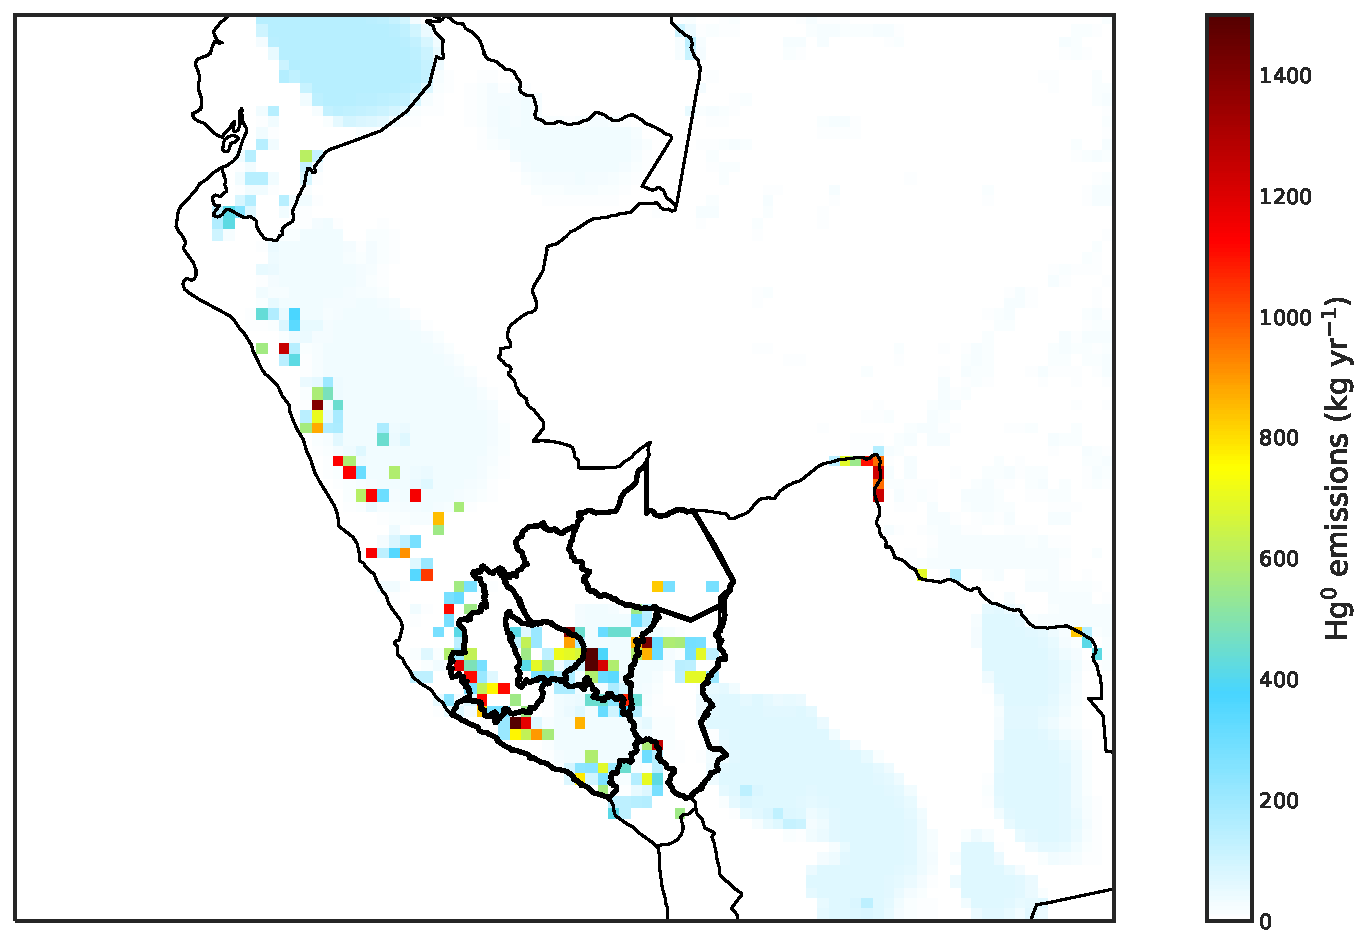
\includegraphics[width = 0.45\linewidth]{templates/figures/Peru_Maps/GMA2018inventory025x025.pdf}} &
\subfloat[GEOS Chem Grid]{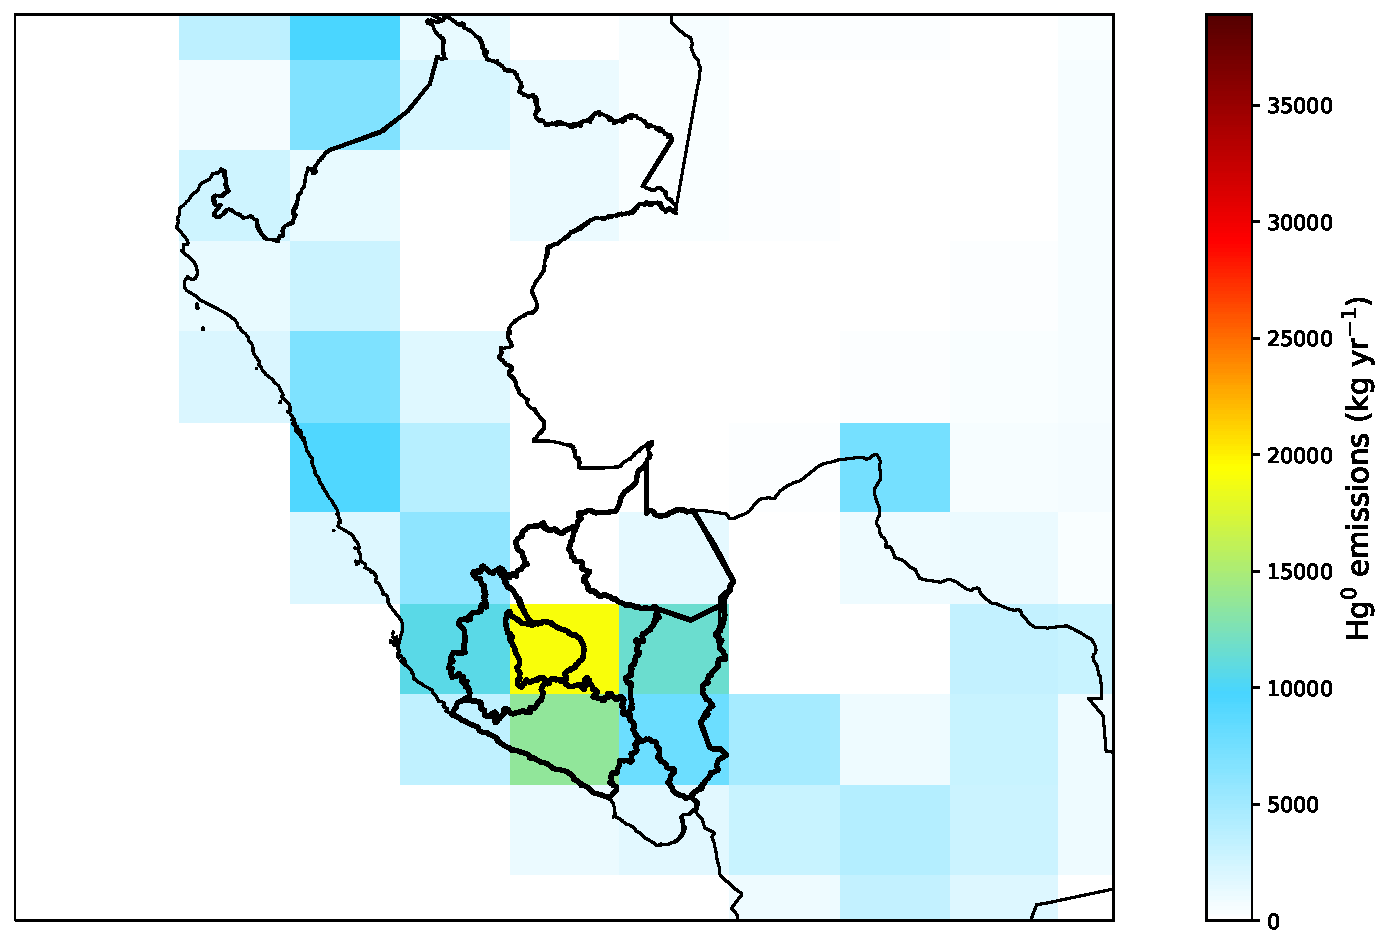
\includegraphics[width = 0.45\linewidth]{templates/figures/Peru_Maps/GMA2018inventory2x25.pdf}}\\


\end{tabular}
  
\centering
\captionof{figure}{Map showing how the GMA2018 emission estimates for the year 2015 were distributed in Peru }
\label{fig:GMA2018}
\end{figure}
\FloatBarrier


\begin{flushleft}
For each grid box in the case study region, the emissions were modified from their original GMA 2018 estimates to new values based on Hg emission estimates produced by the Artisanal Gold Council(AGC)
\end{flushleft}

\subsection{Markov Chain Monte Carlo}

\begin{flushleft}
The Markov-Chain Monte Carlo (MCMC) is a sampling method that is also useful for fitting models to data\cite{hogg_data_2018}. We apply the MCMC to constrain ASGM Hg emissions from the case study region in Peru.The basic idea behind this approach is to compare the generated models to the data. The model is generated by a set of parameters, emissions, and we aim to sample from the set of parameters that best fits our data. The MCMC is used to compare the modelled concentrations to the observed data using metrics such as the $95^{th}$ confidence interval, mean and the interquartile range. The MCMC generatively models given data by sampling around optimum values from the posterior distribution. The MCMC is a Bayesian approach; hence it requires the definition of priors on the parameters of interest. The priors encode information that we already know of the system. The probability of the model given the observed data is given by the posterior probability, $P(\theta|D)$, which is calculated using the Bayes theorem:

\begin{equation}
\label{bayes_eq}
P(\theta|D)=\frac{P(D|\theta)P(\theta)}{P(D)}
\end{equation}
where:
\end{flushleft}

\begin{description}[leftmargin=!,labelwidth={3 em}]
    \item [$P(D|\theta)$] is the likelihood which is the probability of the data given the model
    \item [$P(\theta)$] is the prior which is the probability of the model and 
    \item [$P(D)$] is the evidence which is the probability of the data.
\end{description}

\begin{flushleft}
The MCMC enables the estimation of the sampling of the posterior distribution which is the left-hand side of Equation~\ref{bayes_eq}. The MCMC is set set up by following a set of steps that include defining a function that outputs a model given a set of input parameters and establishing an ensemble of walkers defined by a $\theta$ vector that contains a set of parameters form the model generating function.For the model generating function the Hg concentration at a particular grid box is defined as a linear combination of Hg concentration signals from the case study region and the baseline Hg concentration as shown in the Equation \ref{Hg_conc} below:

\begin{align}
\begin{split}\label{Hg_conc}
Hg_{conc}= {}&Hg_{m(MdD)}+ Hg_{m(S-Puno)} + Hg_{m(N-Puno)} + Hg_{m(Apr)}+ Hg_{m(Aqp)}\\
            & +Hg_{m_0}
\end{split}
\end{align}

where:
\end{flushleft}

\begin{description}[leftmargin=!,labelwidth={5 em}]
    \item [$Hg_{m(MdD)}$] is the Hg concentration signal resulting from emissions from the Madre de Dios (MdD) grid box
    \item [$Hg_{m(S-Puno)}$] is the Hg concentration signal resulting from emissions from the South Puno (S-Puno) grid box
    \item [$Hg_{m(N-Puno)}$] is the Hg concentration signal resulting from emissions from the North Puno (N-Puno) grid box
    \item [$Hg_{m(Apr)}$] is the Hg concentration signal resulting from emissions from the Apurimac (Apr) grid box
    \item [$Hg_{m(Aqp)}$] is the Hg concentration signal resulting from emissions from the Arequipa (Aqp) grid box
    \item [$Hg_{m_0}$] is the baseline Hg concentration signal.
\end{description}

\begin{flushleft}
Each of the $Hg_{m(region)}$ terms of Equation \ref{Hg_conc} represent signals from the different departments are calculated using Equation~\ref{ysignal}. Equation~\ref{ysignal} The $m_(region)$ terms are the only unknowns in  and the equation can be expanded to isolate the terms with $m_(region)$, which is the parameter we are optimizing for in the MCMC method. The expanded form of Equation \ref{Hg_conc} is shown below:

\begin{align}
\begin{split}\label{Cs36PoGd2l}
Hg_{conc}={}& (m_{(MdD)}Hg_{sig_{(MdD)}} -m_oHg_{sig_{(MdD)}})+ (m_{(S-Puno)}Hg_{sig_{(S-Puno)}} -m_oHg_{sig_{(S-Puno)}}) \\
            &+ (m_{(N-Puno)}Hg_{sig_{(N-Puno)}} -m_0Hg_{sig_{(N-Puno)}}) + (m_{(Apr)}Hg_{sig_{(Apr)}} -m_oHg_{sig_{(Apr)}}) \\
            &+ (m_{(Aqp)}Hg_{sig_{(Aqp)}} -m_oHg_{sig_{(Aqp)}})+Hg_{m_0}
\end{split}
\end{align}

Since the values of $m_{(region)}$ are the parameters that we want to estimate using MCMC, they can represented as $\theta_i=m_{(region)}, i=1$ and the other terms including the background concentration are combined into one constant, C:

\begin{equation}
\begin{aligned}
    Hg_{conc}  & = \theta_0C  + \theta_1Hg_{sig_{(MdD)}}+ \theta_2Hg_{sig_{(S-Puno)}} +  \theta_3Hg_{sig_{(N-Puno)}} \\
                & \ \ \ \  +\theta_4Hg_{sig_{(Apr)}} +  \theta_5Hg_{sig_{(Aqp)}}
\end{aligned}
\end{equation}

\begin{align}
Hg_{conc} =\begin{bmatrix} C & Hg_{sig_{(MdD)}} & Hg_{sig_{(S-Puno)}} &Hg_{sig_{(N-Puno)}} &Hg_{sig_{(Apr)}} &Hg_{sig_{(Aqp)}}\end{bmatrix} \times 
            \begin{bmatrix} \theta_0 \\ \theta_1 \\ \theta_2\\ \theta_3\\ \theta_4\\ \theta_5  \end{bmatrix}
\end{align}
where $\theta_0=1$ and $Hg_{conc}$ is the modeled Hg concentration at the observation site of interest.
\end{flushleft}

\begin{flushleft}
The output of 
\end{flushleft}


\subsection{Subsection with list}



\section{Results and Discussion}
\subsection{Markov Chain Monte Carlo Simulation }
\renewcommand{\arraystretch}{2}

    
\begin{table}[H]
\caption{Table showing the emission estimates for each of the grid boxes in the case study region when the $95^{th}$ percentile range is used as the metric to compare the model outputs to observations}
    \label{tab:MCMC_estimates}
\begin{tabular}{lc}

\textbf{Region}        & \textbf{Emission Estimate}                             \\
\hline
Madre de Dios & $16.97^{+21.27}_{-12.27}$ \\

Apurimac      & $14.90^{+16.16}_{-10.53}$\\

Arequipa      & $32.83^{+34.94}_{-24.31}$ \\

North Puno    & $13.44^{+17.51}_{-10.07}$ \\

South Puno    & $06.51^{+7.26}_{-4.72}$ \\
\hline
\end{tabular}
\centering
\end{table}

\begin{figure}[H]
  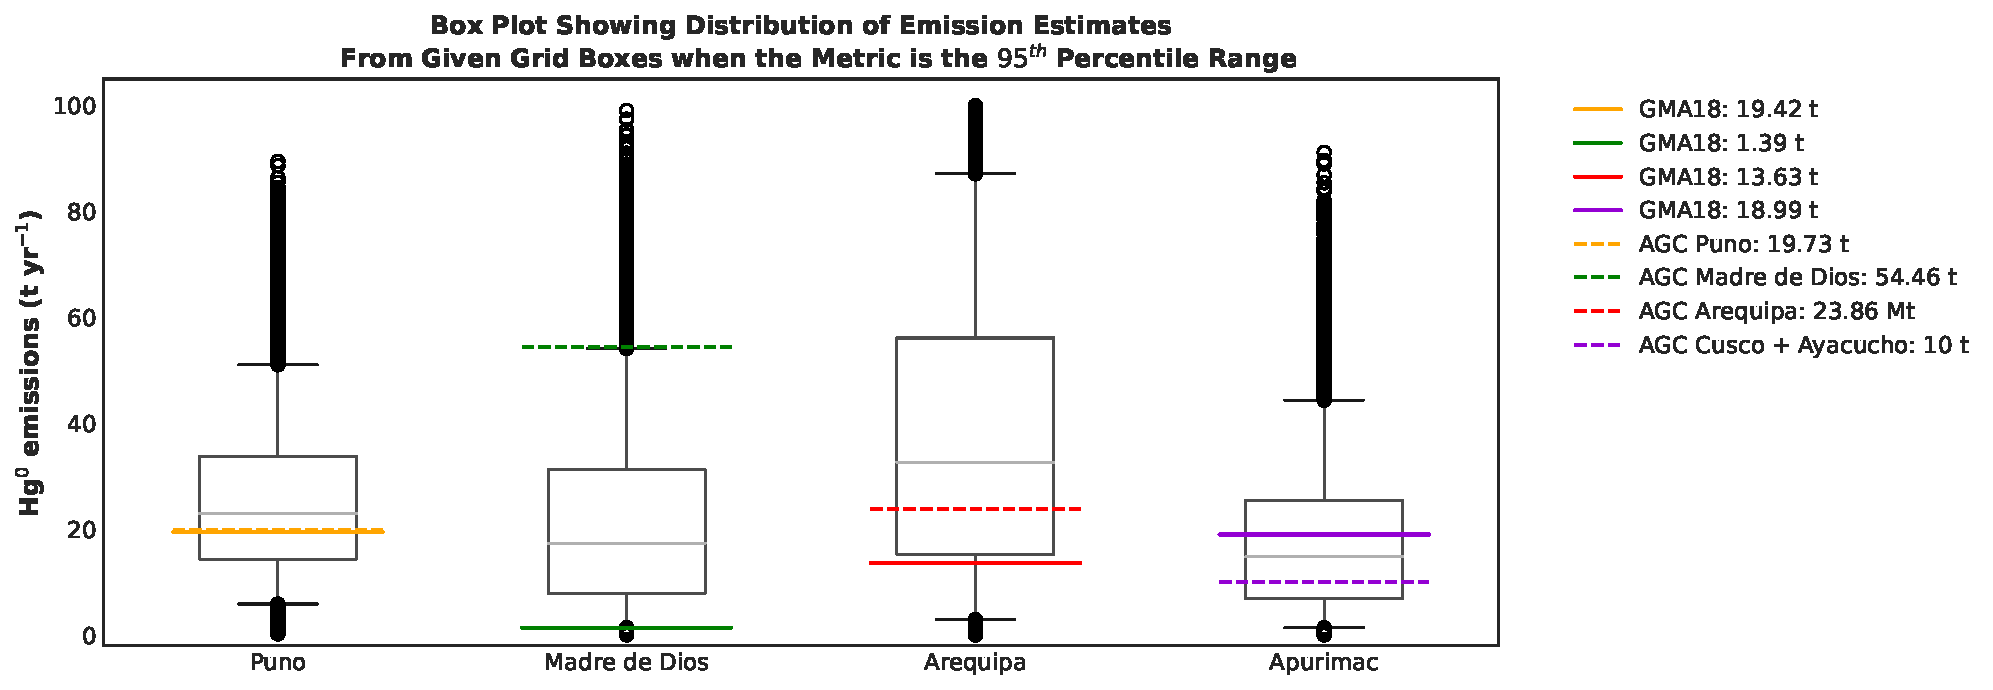
\includegraphics[width=\textwidth]{templates/figures/MCMC/MCMCMCMC_Estimates95th.pdf}
  \centering
  \caption{Emission Estimates when the $95^{th}$ percentile range is used as the metric to compare the model outputs to observations }
  \label{fig:MCMC_estimatesiqr}
\end{figure}
\FloatBarrier

\begin{figure}[H]
  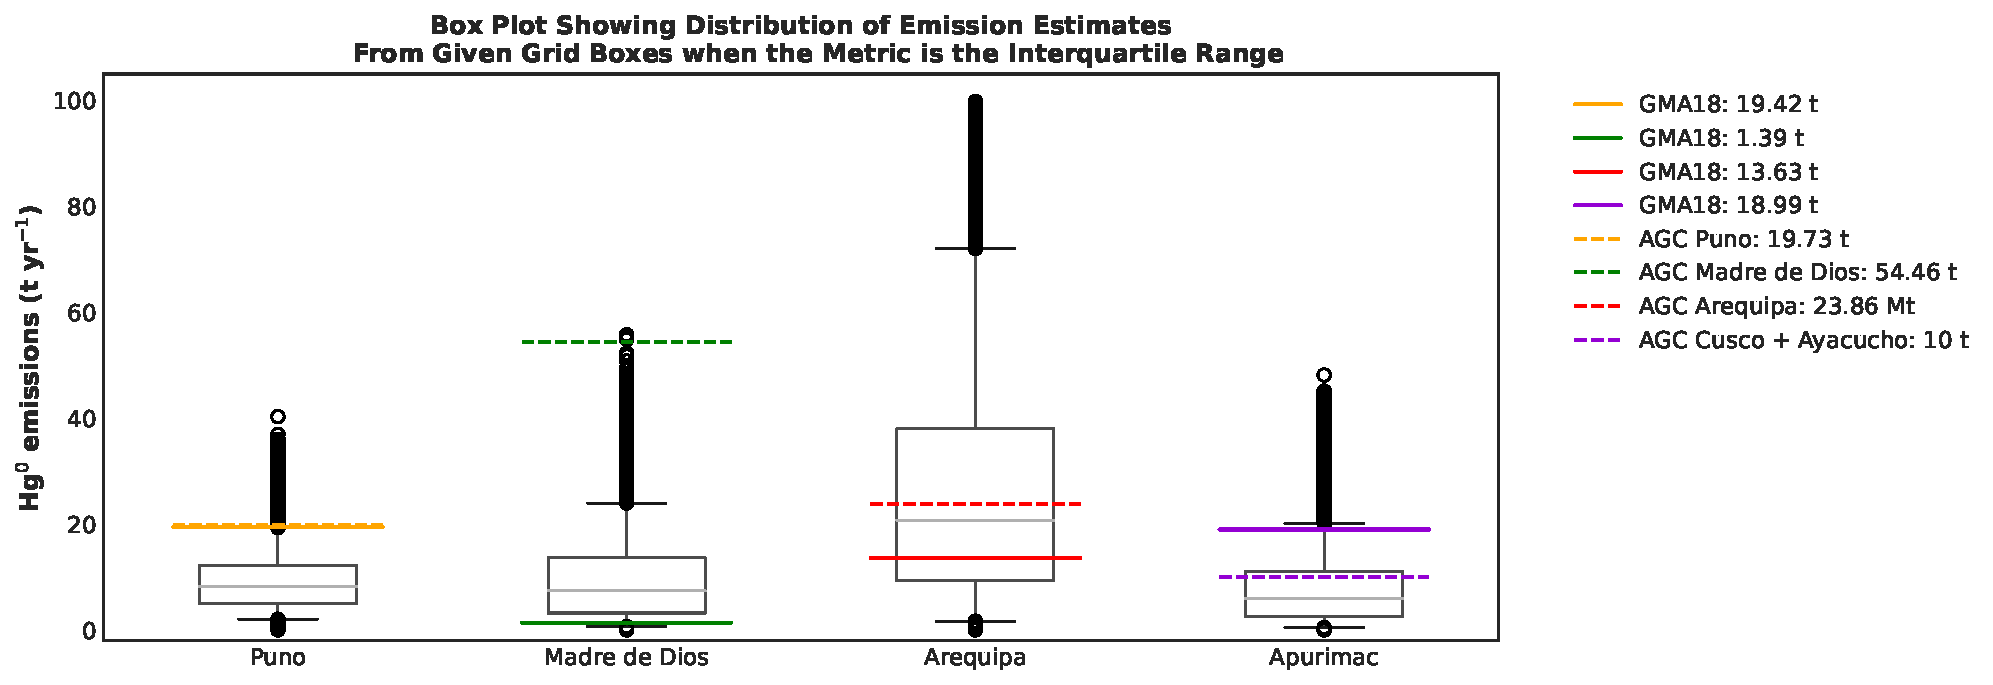
\includegraphics[width=\textwidth]{templates/figures/MCMC/MCMCMCMC_Estimatesiqr.pdf}
  \centering
  \caption{Emission Estimates when the IQR is used as the metric to compare the model outputs to observations }
  \label{fig:MCMC_estimates95}
\end{figure}
\FloatBarrier
\begin{flushleft}

\end{flushleft}



\subsection{Another subsection sample}
\section{Policy Implications}